\documentclass[10pt]{article}

\usepackage[a4paper,margin=0.82in]{geometry}
\usepackage{amsmath,amssymb,amsthm,mathtools}
\usepackage{microtype}
\usepackage{booktabs}
\usepackage{tabularx}
\usepackage{enumitem}
\usepackage{multicol}
\usepackage{xcolor}
\usepackage{tikz}
\usetikzlibrary{arrows.meta,calc,positioning}
\usepackage[colorlinks=true,linkcolor=blue!50!black,
  citecolor=blue!50!black,urlcolor=blue!50!black]{hyperref}

\newtheorem{theorem}{Theorem}
\newtheorem{proposition}[theorem]{Proposition}
\newtheorem{corollary}[theorem]{Corollary}
\theoremstyle{definition}
\newtheorem{definition}[theorem]{Definition}

\newcommand{\C}{\mathbb C}
\newcommand{\R}{\mathbb R}
\newcommand{\N}{\mathbb N}
\newcommand{\T}{\mathbb T}
\newcommand{\HS}{\mathrm{HS}}
\newcommand{\proj}{\mathrm{proj}}
\newcommand{\Fid}{\mathcal F}
\newcommand{\Hwater}{\mathcal H}
\newcommand{\Bhaar}{\mathcal B_{\mathrm H}}
\newcommand{\ee}{\mathrm e}

\title{\textbf{An information law for quantum recurrence}}
\author{Michael Haufschild}
\date{28 July 2026}

\begin{document}
\maketitle

\begin{abstract}
A closed quantum system can return near its initial state, but known guarantees
primarily count energy levels.  We determine the information that a return must
actually synchronize.  For every finite pure state and accuracy, we prove an
exact Haar-quantile bound for the fraction of spectra returning through any
finite horizon, together with a deterministic deadline for every spectrum.
The Haar scale is governed by reverse water filling.  The constructive law may discard
an arbitrary low-weight tail: discarded probability pays amplitude error,
whereas only retained coordinates pay clock dimension.  This removes the
full-support-linear remainder from the refined statement.  For every finite
collection of mixed states or observables, return distance is then exactly a
weighted energy on its coherence graph.  Its visible phase rank is the number
of energy sectors minus the number of coherence components, yielding a
deterministic recurrence deadline with that rank as exponent.  The identity
extends to arbitrary summable pure-point spectra.  Quantum return is therefore
controlled by how coherence is distributed, selected and connected.
\end{abstract}

\noindent\textbf{Summary.}
How long must a quantum system wait to resemble itself again?  The answer is
not fixed by size alone.  Weakly occupied energy levels can be ignored at a
specified accuracy through the same ``water-filling'' rule used to allocate
loss in data compression, while a chosen set of observations sees only a
network of relative phases.  The law below gives finite guarantees for every
allowed phase packet and a quantitative prevalence law over all phase packets.

\section*{Quantum return as an information problem}

Recurrence is the long-time counterpart of reversible microscopic dynamics.
A finite closed quantum system eventually returns near its initial state
\cite{BocchieriLoinger1957}.  Recurrences of selected observables have been
resolved in interacting gases containing thousands of atoms
\cite{RauerEtAl2018}, and a 2026 superconducting-qubit proposal makes their
size scaling experimentally accessible \cite{KarimiEtAl2026}.  Quantitative
theory has meanwhile produced generic recurrence scales
\cite{CamposVenuti2015}, deterministic packing bounds and hard
effective-support refinements \cite{KotowskiOszmaniec2026}, simultaneous
all-state bounds \cite{GuptaShort2026}, and arithmetic criteria for exact
Floquet return \cite{AnandEtAl2026}.

These results leave a basic distinction unresolved.  A state assigns different
probabilities to different energy sectors, and an experiment observes only
selected coherences.  Counting all sectors equally therefore discards two
kinds of information: \emph{how strongly} each phase contributes and
\emph{which relative phases} are visible.  We solve the two questions
separately and then join them.

For pure states, the answer is a continuous, accuracy-dependent water
functional.  For arbitrary finite families of density matrices and
observables, the answer is a coherence network.  The former controls a
universal deadline and every Haar recurrence quantile; the latter gives an
exact return identity, an exact observable phase rank, and a universal finite
deadline.  Figure
\ref{fig:law} shows the two reductions.

\begin{figure}[t]
\centering
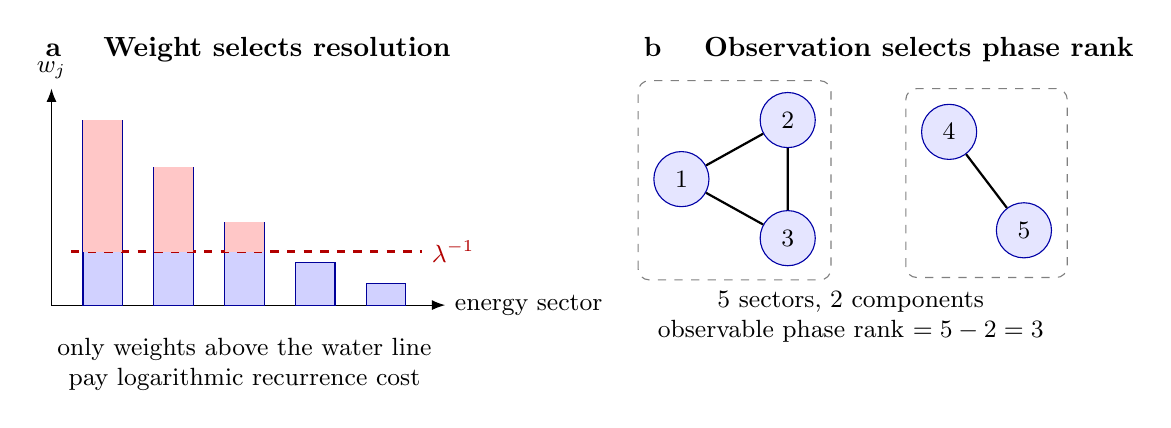
\begin{tikzpicture}[font=\small,>=Latex]
  \node[anchor=west,font=\bfseries] at (-0.2,3.25) {a \quad Weight selects resolution};
  \draw[->] (0,0) -- (0,2.75) node[above] {$w_j$};
  \draw[->] (0,0) -- (5.0,0) node[right] {energy sector};
  \foreach \x/\h in {0.65/2.35,1.55/1.75,2.45/1.05,3.35/0.54,4.25/0.27}{
    \fill[blue!18] (\x-0.25,0) rectangle (\x+0.25,\h);
    \draw[blue!60!black] (\x-0.25,0) rectangle (\x+0.25,\h);
  }
  \draw[dashed,red!70!black,thick] (0.25,0.68) -- (4.7,0.68)
    node[right,red!70!black] {$\lambda^{-1}$};
  \fill[red!22] (0.4,0.68) rectangle (0.9,2.35);
  \fill[red!22] (1.3,0.68) rectangle (1.8,1.75);
  \fill[red!22] (2.2,0.68) rectangle (2.7,1.05);
  \node[align=center] at (2.45,-0.75)
    {only weights above the water line\\pay logarithmic recurrence cost};

  \begin{scope}[xshift=8.0cm]
    \node[anchor=west,font=\bfseries] at (-0.6,3.25)
      {b \quad Observation selects phase rank};
    \tikzset{v/.style={circle,draw=blue!65!black,fill=blue!10,
      minimum size=7mm,inner sep=0pt}}
    \node[v] (a) at (0,1.6) {$1$};
    \node[v] (b) at (1.35,2.35) {$2$};
    \node[v] (c) at (1.35,0.85) {$3$};
    \node[v] (d) at (3.4,2.2) {$4$};
    \node[v] (e) at (4.35,0.95) {$5$};
    \draw[thick] (a)--(b) (a)--(c) (b)--(c);
    \draw[thick] (d)--(e);
    \draw[dashed,rounded corners,gray] (-0.55,0.32) rectangle (1.9,2.85);
    \draw[dashed,rounded corners,gray] (2.85,0.35) rectangle (4.9,2.75);
    \node[align=center] at (2.15,-0.15)
      {$5$ sectors, $2$ components\\observable phase rank $=5-2=3$};
  \end{scope}
\end{tikzpicture}
\caption{\textbf{Two information reductions.}
\textbf{a}, Reverse water filling chooses the phase resolution demanded from
each spectral probability.  Modes below the water line are inactive in the
leading functional.  \textbf{b}, A state or observable sees an edge only when
it contains coherence between the corresponding energy sectors.  One common
phase per connected component is invisible.}
\label{fig:law}
\end{figure}

\section*{A rate--distortion law for every finite pure state}

Let a pure state have positive spectral probabilities
\[
 w=(w_1,\ldots,w_r),\qquad w_j>0,\qquad \sum_{j=1}^r w_j=1,
\]
on its support.  Under one step of a diagonal Floquet unitary with eigenphases
\(\omega=(\omega_1,\ldots,\omega_r)\), its return amplitude and fidelity after
\(n\) steps are
\begin{equation}
 A_w(n;\omega)=\left|\sum_{j=1}^r w_j\ee^{in\omega_j}\right|,
 \qquad
 \Fid_w(n;\omega)=A_w(n;\omega)^2.
 \label{eq:amplitude}
\end{equation}
Choose a pivot \(k\), which absorbs the physically irrelevant common phase.
Allocate distortions \(D_j\) to the remaining coordinates and define
\begin{align}
 \Hwater_k(w,\eta)
 &=\min\left\{\frac12\sum_{j\ne k}\log\frac{w_j}{D_j}:
       0<D_j\leq w_j,\ \sum_{j\ne k}D_j\leq\eta\right\}, \label{eq:Hk}\\
 \Hwater_{\proj}(w,\eta)&=\min_k\Hwater_k(w,\eta).
 \label{eq:Hproj}
\end{align}
If \(\eta\geq1-w_k\), then \(\Hwater_k=0\) and we set \(\lambda_k=1\).
Otherwise choose a water level \(\lambda_k>0\) satisfying
\begin{equation}
 \sum_{j\ne k}\min\{w_j,\lambda_k^{-1}\}=\eta,
 \label{eq:waterlevel}
\end{equation}
and the exact optimizer is
\begin{equation}
 D_j^*=\min\{w_j,\lambda_k^{-1}\},\qquad
 \Hwater_k(w,\eta)=\frac12\sum_{j\ne k}\log_+(\lambda_k w_j).
 \label{eq:waterfill}
\end{equation}
Equations \eqref{eq:Hk}--\eqref{eq:waterfill} are numerically the parallel
Gaussian reverse-water-filling program \cite{CoverThomas2006,GrayNeuhoff1998}.
We claim equality of finite convex programs, not an operational source code:
there is no random source or communication channel in
\eqref{eq:amplitude}.
Rate--distortion also controls approximate block-match recurrence in
stationary random sources \cite{KanayaMuramatsu1997}; that asymptotic
random-string theorem is distinct from the finite projective phase problem
here.

Define the pivot-resolved Haar budget
\begin{equation}
 \Bhaar(w,\eta)=
 \sum_{k=1}^r
 \exp\!\left\{\frac{\pi}{4}\lambda_k\eta
 -\Hwater_k(w,\eta)\right\}.
 \label{eq:Bhaar}
\end{equation}
For a chosen non-pivot set \(S\), let
\(\tau_S=\sum_{j\ne k,\,j\notin S}w_j\).  Coordinates outside \(S\) will not
be synchronized.

\begin{theorem}[Universal and typical recurrence law]
\label{thm:water}
For every finite probability vector on a support of size \(r\geq2\), every
\(0<\eta\leq1\), and every \(N\geq1\), normalized Haar measure \(m_{\T^r}\)
satisfies
\begin{equation}
\boxed{
 m_{\T^r}\!\left\{\omega:\exists\,1\leq n\leq N,\,
   \Fid_w(n;\omega)\geq(1-\eta)^2\right\}
 \leq N\Bhaar(w,\eta).}
\label{eq:quantile-law}
\end{equation}
Moreover, for every pivot \(k\), selected set
\(S\subseteq\{1,\ldots,r\}\setminus\{k\}\), and allocations
\(0<D_j\leq w_j\) satisfying
\begin{equation}
 2\tau_S+\sum_{j\in S}D_j\leq\eta,
 \label{eq:selected-feasible}
\end{equation}
every phase packet returns by a deadline \(P_S\) obeying
\begin{equation}
\boxed{
 P_S=\prod_{j\in S}
 \left\lceil\pi\sqrt{\frac{2w_j}{D_j}}\right\rceil,
 \qquad
 \log P_S\leq
 \frac12\sum_{j\in S}\log\frac{w_j}{D_j}
 +|S|\log(2\pi\sqrt2).}
\label{eq:selected-ceiling}
\end{equation}
\end{theorem}

Thus, if \(N\Bhaar\leq\alpha\), at least a fraction \(1-\alpha\) of spectra
avoid the target through \(N\); the lower statement is a population law, not
one adversarial spectrum.  Conversely, \eqref{eq:selected-ceiling} works for
every spectrum.  Discarded modes pay the worst-case amplitude loss
\(2\tau_S\), but no clock factor.  The exact product in
\eqref{eq:selected-ceiling} has no additive dimension remainder; its simpler
logarithmic envelope charges a rounding constant only on the chosen set \(S\).

For comparison, define \(T_w(\eta)\) as the least positive integer \(N\) such
that every phase packet has some return by that deadline:
\begin{equation}
 \forall\omega\in\R^r\quad \exists\,1\leq n\leq N:
 \quad \Fid_w(n;\omega)\geq(1-\eta)^2.
 \label{eq:minimax-time}
\end{equation}
This worst-packet quantity is no longer the organizing statement.  It remains
a useful coarse corollary:
\begin{equation}
 \Hwater_{\proj}(w,\eta)-\frac{\pi}{4}(r-1)-\log(2r)
 <\log T_w(\eta)
 \leq
 \Hwater_{\proj}(w,\eta)+(r-1)\log(2\pi\sqrt2).
\label{eq:waterlaw}
\end{equation}
Its dimension-linear terms arise by synchronizing every non-pivot coordinate
and replacing every pivot-specific factor in \eqref{eq:Bhaar} by its
worst-case envelope.  They are not the refined law.

The distinction from hard support is exact even for two levels.  Put
\[
 \varepsilon_\eta=\sqrt{2\eta-\eta^2},\qquad
 \delta_\eta=\varepsilon_\eta/2,
\]
and take \(0<\eta<2/5\), \(q>1\), and \(q\delta_\eta<1/2\).  Both
\[
 w_\eta=(1-q\delta_\eta,q\delta_\eta),\qquad u=(1/2,1/2)
\]
require two coordinates at tail tolerance \(\delta_\eta\), but
\begin{equation}
 \Hwater_{\proj}(w_\eta,\eta)
 =\frac12\log\frac{q\delta_\eta}{\eta}
 <\frac12\log\frac{1}{2\eta}
 =\Hwater_{\proj}(u,\eta).
\label{eq:support-separation}
\end{equation}
Thus a hard effective support does not determine the weight-sensitive
functional at the same operational accuracy.

\section*{Every finite observer has a coherence network}

The pure-state law answers how probabilities allocate phase resolution.  A
mixed state or a restricted measurement family poses a second question:
which phase differences are visible at all?

Let \(E_1,\ldots,E_d\) be the distinct energy sectors of a finite Hamiltonian,
\(z_i(t)=\ee^{itE_i}\), and let \(B^{(a)}\), \(a\in J\), be any finite family
of matrices with observation weights \(\lambda_a\geq0\).  The matrices may be
density operators, Heisenberg observables after reversing the phase
orientation, or both.  Define
\begin{align}
 D^2(t)&=\sum_{a\in J}\lambda_a
   \left\|U_tB^{(a)}U_t^\dagger-B^{(a)}\right\|_{\HS}^2,
 \label{eq:observer-distance}\\
 W_{ij}&=\sum_{a\in J}\lambda_a|B^{(a)}_{ij}|^2.
 \label{eq:observer-weight}
\end{align}
The observer coherence graph \(G\) has vertices \(1,\ldots,d\) and an
undirected edge \(\{i,j\}\) exactly when \(i\ne j\) and
\(W_{ij}>0\) or \(W_{ji}>0\).  Let \(c(G)\) be its number of connected
components, including isolated vertices.

\begin{theorem}[Universal observer-coherence law]
\label{thm:graph}
For every finite Hamiltonian, every finite matrix family and all nonnegative
observation weights,
\begin{equation}
\boxed{
 D^2(t)=\sum_{i,j}W_{ij}
 \left|z_i(t)\overline{z_j(t)}-1\right|^2.}
\label{eq:phase-energy}
\end{equation}
Consequently:
\begin{enumerate}[leftmargin=2.1em,label=(\roman*)]
 \item \(D(t)=0\) if and only if \(z_i(t)=z_j(t)\) on every edge of \(G\),
 equivalently, the phase is constant on every connected component;
 \item the real dimension of the visible relative-phase space is exactly
 \begin{equation}
   \operatorname{rank}_{\rm obs}=d-c(G);
   \label{eq:graph-rank}
 \end{equation}
 \item for every integer resolution \(Q\geq1\), some positive integer
 \(n\) satisfies
 \begin{align}
  n&\leq(Q+1)^{\,d-c(G)}, \label{eq:graph-deadline}\\
  D^2(n)&\leq
    4\left(\frac{2\pi}{Q+1}\right)^2\sum_{i,j}W_{ij}.
  \label{eq:graph-error}
 \end{align}
\end{enumerate}
\end{theorem}

The exponent in \eqref{eq:graph-deadline} is the exact number of visible phase
coordinates, not the Hilbert-space dimension.  Adding an observer changes the
rank only if its nonzero energy-basis blocks connect previously disconnected
components.  A diagonal state has no edges and is stationary.  A fully
connected coherence pattern pays \(d-1\) relative phases.  Between them, every
graph topology is handled by the same theorem.

Equations \eqref{eq:graph-deadline}--\eqref{eq:graph-error} are a guaranteed
horizon, not a claim that every fixed Hamiltonian saturates it.  Arithmetic
relations among its energy gaps can make return earlier.  This qualification
is essential: graph topology fixes observable phase capacity, while the
particular spectrum fixes the orbit inside that capacity.

\section*{The exact law survives infinite pure-point spectra}

The identity itself is not finite-dimensional.  Let \(\iota\) be an arbitrary
pure-point spectral index, let \(J\) be an arbitrary observer family, and let
\(B^{(a)}_{ij}\) be blocks in any complex normed space.  Whenever the
nonnegative series below is summable,
\begin{equation}
 D^2(t)=\sum_{a,i,j}\lambda_a\|B^{(a)}_{ij}\|^2
  \left|\ee^{it(E_i-E_j)}-1\right|^2.
\label{eq:purepoint}
\end{equation}
Moreover,
\begin{equation}
 D(t)=0
 \quad\Longleftrightarrow\quad
 \ee^{it(E_i-E_j)}=1
\quad\text{for every }\lambda_a>0\text{ and }B^{(a)}_{ij}\ne0.
\label{eq:purepoint-zero}
\end{equation}
This gives a dimension-free necessary-and-sufficient law for exact
observer return.  It deliberately does not assert a uniform finite deadline
for continuous spectra, where recurrence need not occur.  The finite deadline
and the infinite identity are different conclusions, and
\eqref{eq:purepoint}--\eqref{eq:purepoint-zero} state the exact boundary.

\section*{Local clock quality does not determine global return}

The coherence carrier cannot be replaced by familiar local summaries.  An
explicit three-level pair demonstrates this.  Let the common Hamiltonian have
energies
\[
 (E_0,E_1,E_2)=(0,1,\sqrt2),\qquad \delta=\sqrt2-1,
\]
and define population packets
\[
 p=(1-\delta,\delta,0),\qquad
 q=(1-2\delta,\delta,\delta).
\]
For normalized kets with these energy probabilities, put
\begin{equation}
 \rho_p=\frac16 I+\frac12|\psi_p\rangle\!\langle\psi_p|,
 \qquad
 \rho_q=\frac16 I+\frac12|\psi_q\rangle\!\langle\psi_q|.
\label{eq:qutrit-states}
\end{equation}
Both states are full rank and have the complete density spectrum
\(\{2/3,1/6,1/6\}\).  They have the same nonzero initial squared
Hilbert--Schmidt speed and the same symmetric-logarithmic-derivative quantum
Fisher information for elapsed time.  The equality follows from the exact
variance identity
\begin{equation}
 \operatorname{Var}_{p}(E)=\operatorname{Var}_{q}(E).
\label{eq:variance-equality}
\end{equation}
Nevertheless, at the common ticks \(t=2\pi n\), \(\rho_p\) returns exactly
for every \(n\), whereas \(\rho_q\) never returns exactly at a positive tick.
Writing \(R_q(n)\) for one half of the square root of its pure-spike fidelity
defect, one has for every \(n\geq1\)
\begin{equation}
 \frac{\sqrt{\delta(1-\delta)}}{2n}\leq R_q(n),
\label{eq:qutrit-lower}
\end{equation}
and for every \(Q\geq1\) there is \(1\leq n\leq Q\) with
\begin{equation}
 R_q(n)\leq\frac{\pi\sqrt{\delta(1-\delta)}}{Q}.
\label{eq:qutrit-upper}
\end{equation}
Hence equal state spectrum, initial speed and optimal local timing precision
coexist with exact periodicity for one clock and an inverse-resolution law
for the other.  The missing information is relational: which energy gaps the
state coherently occupies.

\section*{Experimental discriminator}

Theorems \ref{thm:water} and \ref{thm:graph} separate two controls already
available in recurrence platforms: state preparation changes spectral
weights, while probe choice changes the coherence graph.  A direct protocol
is therefore:
\begin{enumerate}[leftmargin=2.1em]
 \item calibrate a stroboscopic unitary and prepare states with known
 energy-basis weights;
 \item choose a family of tomographic blocks or observables whose union graph
 has prescribed component count;
 \item measure the weighted Hilbert--Schmidt displacement through
 \((Q+1)^{d-c(G)}\) ticks.
\end{enumerate}
Ideal unitary dynamics must contain a tick satisfying
\eqref{eq:graph-error}.  Changing only the observer family can reduce the
guaranteed exponent by increasing \(c(G)\); changing only weak spectral
weights changes the water allocation without changing hard support.  The
multiqubit recurrence blueprint of Ref.~\cite{KarimiEtAl2026} supplies a
finite-level setting, while the observable-selective many-body recurrence of
Ref.~\cite{RauerEtAl2018} supplies the complementary motivation: a large
system can recur for one probe and not visibly recur for another on the same
window.

\section*{Discussion}

The results answer a single question at three levels:
\[
\begin{array}{c}
\text{How much phase information must a return synchronize?}\\[2mm]
\text{pure state: reverse-water-filled spectral weights}\\
\text{finite observer family: }d-c(G)\text{ connected relative phases}\\
\text{arbitrary pure-point family: every visible block phase}.
\end{array}
\]
This classification is universal over the stated closed, unitary,
pure-point setting.  It does not infer cosmology, gravity, information loss
or an arrow of time.  Those subjects require additional physical structure
absent from the hypotheses.

The cross-disciplinary point is exact but limited: recurrence and parallel
Gaussian rate--distortion share the same finite optimization problem.  The
quantum theorem supplies a finite-horizon Haar population law and a
spectrum-uniform construction; it does not turn a Floquet system into a
communication channel.  The graph law then shows why no scalar entropy can be
a complete recurrence invariant: connectivity of observable coherence is
independent information.

Together, the laws replace a dimension-only picture by an
observer-sensitive one.  Quantum systems remember how to return through the
weights and connectivity of the coherences that are asked to return.

\section*{Methods}

\subsection*{Reverse-water-filling optimizer}

For a fixed pivot, set \(x_j=w_j/D_j\).  The feasible set in
\eqref{eq:Hk} becomes
\[
 x_j\geq1,\qquad \sum_{j\ne k}\frac{w_j}{x_j}\leq\eta,
\]
and the objective is \(\frac12\sum_{j\ne k}\log x_j\).  If
\(\eta<1-w_k\), continuity gives a level \(\lambda_k\) solving
\eqref{eq:waterlevel}.  The candidate
\(x_j^*=\max\{1,\lambda_kw_j\}\) is feasible.  Global optimality follows by
summing the one-coordinate supporting inequality
\[
 \log\max\{1,\lambda a\}
 +\lambda\!\left(\min\{a,\lambda^{-1}\}-\frac{a}{x}\right)
 \leq\log x,\qquad x\geq1.
\]
This proves \eqref{eq:waterfill}.

\subsection*{Selected-support recurrence ceiling}

Fix \(k,S,D\) as in \eqref{eq:selected-feasible}, set
\(x_j=w_j/D_j\), and put
\[
 Q_j=\left\lceil\pi\sqrt{2x_j}\right\rceil,\qquad
 P_S=\prod_{j\in S}Q_j.
\]
Use one box on every discarded coordinate and partition each selected phase
circle into \(Q_j\) arcs.  Two of the \(P_S+1\) orbit points occupy the same
product box.  Their difference gives \(1\leq n\leq P_S\) and centered
selected errors \(|\theta_j|\leq2\pi/Q_j\).  Every discarded phasor has real
part at least \(-1\), while \(\cos u\geq1-u^2/2\) on \(S\).  Therefore
\[
 A_w(n;\omega)\geq1-2\tau_S-\frac12\sum_{j\in S}w_j\theta_j^2
 \geq1-2\tau_S-\sum_{j\in S}\frac{w_j}{x_j}\geq1-\eta.
\]
Using \(Q_j\leq2\pi\sqrt{2x_j}\) proves
\eqref{eq:selected-ceiling}.  Taking \(S\) to be every non-pivot coordinate
recovers the upper half of \eqref{eq:waterlaw}.

\subsection*{Haar quantiles and the minimax corollary}

For independent Haar phases \(z_j\), set \(m=\sum_jw_jz_j\).  The identity
\[
 \sum_{i,j}w_iw_j|z_i-z_j|^2=2(1-|m|^2)
\]
implies that \(|m|\geq1-\eta\) lies in a union of \(r\) pivot events.  A
Haar-preserving projective shear, exponential Markov inequality, and
\[
 \int_{\T}\exp(-u|z-1|^2)\,dz
 \leq\min\!\left\{1,\frac{\sqrt\pi}{4\sqrt u}\right\}
\]
give the pivot-resolved one-step target bound
\[
 \mu_w(\eta)\leq
 \sum_k\exp\!\left\{\frac{\pi}{4}\lambda_k\eta
 -\Hwater_k(w,\eta)\right\}=\Bhaar(w,\eta).
\]
Every power map preserves Haar measure, so the first \(N\) return targets
have union measure at most \(N\Bhaar(w,\eta)\), proving
\eqref{eq:quantile-law}.  Finally,
\(\lambda_k\eta\leq r-1\) and
\(\Hwater_{\proj}\leq\Hwater_k\) give
\(\Bhaar\leq r\exp\{\pi(r-1)/4-\Hwater_{\proj}\}\).
Choosing \(N\) below half the reciprocal coarse bound leaves a phase packet
outside the union and recovers the lower half of \eqref{eq:waterlaw}.

\subsection*{Observer graph identity and deadline}

In the energy basis,
\[
 (U_tB^{(a)}U_t^\dagger-B^{(a)})_{ij}
 =(z_i\overline z_j-1)B^{(a)}_{ij}.
\]
Summing squared entry norms proves \eqref{eq:phase-energy}.  Every summand is
nonnegative.  It vanishes exactly when every positively weighted nonzero
block has \(z_i=z_j\), which propagates along graph paths.  The space of edge
phase differences is the range of the graph coboundary; choosing one root
per connected component gives rank \(d-c(G)\).

Apply simultaneous phase approximation only to the \(d-c(G)\) non-root
relative energies.  Some \(1\leq n\leq(Q+1)^{d-c(G)}\) places every such
phase within \(2\pi/(Q+1)\) of an integer multiple of \(2\pi\).  Each edge
error is a difference of two root-relative errors and is at most
\(2(2\pi/(Q+1))\).  Multiplication by \(W_{ij}\), squaring and summing proves
\eqref{eq:graph-error}.

\subsection*{Pure-point extension and qutrit separation}

The block identity
\[
 \|\alpha B-B\|^2=\|B\|^2|\alpha-1|^2
\]
holds in every complex normed space.  Summing it proves
\eqref{eq:purepoint}; nonnegativity and summability make a zero sum
equivalent to termwise phase locking, proving \eqref{eq:purepoint-zero}.

For the qutrit pair, \(\delta^2+2\delta=1\) gives
\(\operatorname{Var}_p(E)=\operatorname{Var}_q(E)\).  The spectrum of
\(\frac16I+\frac12|\psi\rangle\langle\psi|\) is independent of the unit
vector \(\psi\), and both local timing quantities are fixed multiples of
this energy variance.  At \(2\pi n\), the only nontrivial phase for
\(\rho_q\) is \(\ee^{2\pi in\sqrt2}\).  The elementary quadratic norm
\[
 1\leq|2n^2-m^2|
 =|n\sqrt2-m|\,|n\sqrt2+m|
\]
for the nearest integer \(m\) gives the inverse-\(n\) lower bound.
One-dimensional Dirichlet approximation gives the matching
inverse-\(Q\) upper bound.  The constants reduce to
\eqref{eq:qutrit-lower}--\eqref{eq:qutrit-upper}.

\section*{Data availability}

No datasets were generated or analysed in this theoretical study.

\section*{Competing interests}

The author declares no competing interests.

\section*{Use of generative artificial intelligence}

Generative language models assisted literature triage, proof exploration and
draft preparation.  The human author takes responsibility for the final
manuscript, mathematical arguments, citations and conclusions.

\begin{multicols}{2}
\begin{thebibliography}{99}
\footnotesize
\setlength{\itemsep}{0.08em}

\bibitem{BocchieriLoinger1957}
P.~Bocchieri and A.~Loinger,
Quantum recurrence theorem,
\emph{Phys. Rev.} \textbf{107}, 337--338 (1957).
\href{https://doi.org/10.1103/PhysRev.107.337}
{doi:10.1103/PhysRev.107.337}.

\bibitem{RauerEtAl2018}
B.~Rauer, S.~Erne, T.~Schweigler, F.~Cataldini, M.~Tajik and
J.~Schmiedmayer,
Recurrences in an isolated quantum many-body system,
\emph{Science} \textbf{360}, 307--310 (2018).
\href{https://doi.org/10.1126/science.aan7938}
{doi:10.1126/science.aan7938}.

\bibitem{KarimiEtAl2026}
B.~Karimi, X.~Wu, A.~N.~Cleland and J.~P.~Pekola,
Blueprint for experiments exploring the quantum recurrence theorem on a
coupled multiqubit system,
\emph{Phys. Rev. Research} \textbf{8}, L012062 (2026).
\href{https://doi.org/10.1103/wv9h-x14y}
{doi:10.1103/wv9h-x14y}.

\bibitem{CamposVenuti2015}
L.~Campos Venuti,
The recurrence time in quantum mechanics,
arXiv:\href{https://arxiv.org/abs/1509.04352}{1509.04352} (2015).

\bibitem{KotowskiOszmaniec2026}
M.~Kotowski and M.~Oszmaniec,
Tight bounds on recurrence time in closed quantum systems,
\emph{Phys. Rev. Lett.}, accepted 23 June 2026.
\href{https://doi.org/10.1103/crwj-qfw5}{doi:10.1103/crwj-qfw5};
arXiv:\href{https://arxiv.org/abs/2601.10409}{2601.10409v2}.

\bibitem{GuptaShort2026}
C.~Gupta and A.~J.~Short,
Recurrence time for finite quantum systems,
\emph{Phys. Rev. A} \textbf{114}, 012208 (2026).
\href{https://doi.org/10.1103/kkz3-fthm}{doi:10.1103/kkz3-fthm}.

\bibitem{AnandEtAl2026}
A.~Anand, D.~Valluri, J.~Davis and S.~Ghose,
Quantum recurrences and the arithmetic of Floquet dynamics,
\emph{Quantum} \textbf{10}, 2074 (2026).
\href{https://doi.org/10.22331/q-2026-04-20-2074}
{doi:10.22331/q-2026-04-20-2074}.

\bibitem{CoverThomas2006}
T.~M.~Cover and J.~A.~Thomas,
\emph{Elements of Information Theory}, 2nd ed. (Wiley, 2006).

\bibitem{GrayNeuhoff1998}
R.~M.~Gray and D.~L.~Neuhoff,
Quantization,
\emph{IEEE Trans. Inf. Theory} \textbf{44}, 2325--2383 (1998).
\href{https://doi.org/10.1109/18.720541}{doi:10.1109/18.720541}.

\bibitem{KanayaMuramatsu1997}
F.~Kanaya and J.~Muramatsu,
An almost sure recurrence theorem with distortion for stationary ergodic
sources,
\emph{IEICE Trans. Fundamentals} \textbf{E80-A}, 2264--2267 (1997).

\end{thebibliography}
\end{multicols}

\end{document}
